\documentclass[conference]{IEEEtran}
% Some Computer Society conferences also require the compsoc mode option,
% but others use the standard conference format.
%
% If IEEEtran.cls has not been installed into the LaTeX system files,
% manually specify the path to it like:
% \documentclass[conference]{../sty/IEEEtran}

% *** CITATION PACKAGES ***
%
\usepackage{cite}
\usepackage{graphicx}

% correct bad hyphenation here
\hyphenation{op-tical net-works semi-conduc-tor}

\begin{document}

%
% paper title
	
\title{Team Prediction in the English Premier League\\ {\large SENG 474}}

\author{%
  Alastair Beaumont\\University of Victoria\\a.beaumont11@gmail.com
  \and Kolby Chapman\\University of Victoria\\kol.j63@gmail.com
  \and Graeme Nathan\\University of Victoria\\graemenathan@gmail.com
  \and Cole Peterson\\University of Victoria\\colpeterson@gmail.com
}

% make the title area
\maketitle

% As a general rule, do not put math, special symbols or citations
% in the abstract
% For peerreview papers, this IEEEtran command inserts a page break and
% creates the second title. It will be ignored for other modes.
\IEEEpeerreviewmaketitle

\section{Introduction}
The English Premier League (EPL) is the highest level of men’s professional soccer in the United Kingdom. In this project we employed data mining techniques to both predict the outcome of games throughout the EPL’s season, as well as to delve into what, if any, affect the threat of relegation has on teams in the league.

Relegation is used in the EPL as a means to change the membership of the league. Teams are ranked by the amount of points the have amassed. These points are gained — never lost — during the season through either the winning or tying of matches. At the end of the season the three teams with the lowest points are swapped out of the league.  
In this paper we explore the predictive power of the threat of relegation on teams in the EPL, and the potential for using data mining techniques to successfully predict match outcomes.

\section{Related work}
Predicting sports performance is a well studied field. Recently, fantasy sport websites like FanDuel and Draft Kings have opened up new gambling opportunities where machine learning techniques can be applied to predict positive returns\cite{Sugar:aa}, and there has been increased interest in the area\cite{Bishop:2004aa} as the industry grows and becomes more profitable. Sports have valued data mining techniques as it helps eliminate the high emotional stakes the field carries for many of its experts which tend to bias predictions\cite{Haghighat:2013aa}. Sport results can have tremendous world-wide impact, the results of soccer matches have even been shown to affect stock investor behaviour\cite{Edmans:2007aa}, and so accurate prediction can be incredibly valuable outside of the stadium. Most research has investigated predicting the outcome of matches, but now there has been emphasis on selecting a fantasy lineup. Other areas of research include using biomechanical measures to gauge player health and fitness to negotiate contract deals\cite{Davenport:2010aa}, and gauge injury risk \cite{Carling:2012aa,Owen:2015aa}, or examine the impact of mid-season changes to the coaching staff\cite{coach}, all of which can help make better predictions of game outcome, or select better players for a lineup.

Sports data exhibits interesting paradoxes where classic gambling fallacies such as the ``hot-hand'' fallacy actually turn out be real, due to the psychological element of sport. Although the authors of \cite{Gilovich:1985aa} found that in general making one basketball shot did not increase your chances of making another, some baseball players were found to be more ``streaky'' than could be statistically accounted for in \cite{Albert:2008aa}. Making more accurate predictions may rely upon teasing apart some of these more complicated and unintuitive elements of sport data, and verifying conventional wisdom like ``home-field advantage'' is legitimate\cite{textbook}. Identifying the right features to use in training a machine learning model for sport can be tricky. Some approaches have relied upon expert opinion to select features\cite{Zdravevski:2010aa}, while others have added single features iteratively, only keeping them if they increased prediction accuracy\cite{Buursma:2011aa}. Within the game of basketball, a team's performance in the area under the net (short shots and rebounds) was found to have the higher impact on final result than performance anywhere else on the court\cite{Ivankovic:2010aa}. As statistics of soccer tend to be relatively sparse compared to other sports, much effort to apply data mining techniques to the game of soccer have relied upon automated processing of video to detect events in matches\cite{Sykora2015,goal_detection}, player speed \cite{Redwood-Brown:2012aa}, or more complex data like player position on the pitch to discover offensive patterns \cite{offence_patterns}. 

 Many classification techniques have been experimented with including Support Vector Machines \cite{Cao:2012aa}, Neural Networks\cite{McCabe:2008aa}, Bayesian Methods\cite{Buursma:2011aa}, Logistic Regression\cite{Cao:2012aa,Buursma:2011aa}, Fuzzy Models\cite{Trawinski:2010aa}, Decision Trees\cite{Zdravevski:2010aa}, and Markov chain Monte Carlo Methods \cite{Rue:2000aa}. It can be difficult to compare the success of these models in different studies because most of them use different data. Additionally, some studies aim to predict binary win/loss, whereas others \cite{Rotshtein:2005aa} classify with margin of victory granularity. Many different methods have shown to have statistically significant predictive powers, with some studies reporting prediction accuracy $>80\%$\cite{Ivankovic:2010aa}. There remains no consensus or conclusion over which methods provide the highest accuracy for sports in general, or the game of soccer. One study \cite{Cao:2012aa} found logistic classifiers, naive Bayes, support vector machines, and artificial neural networks to all produce accuracy of $66.82\% \pm 1.00\%$, demonstrating that no method is clearly better over another on the same data.

\section{Data and Project Description}
The data used for this project was the team stats of soccer teams. These stats include the win/loss record for the team, which team was the home team, the goals scored by each team in the game, and the team's place in the standings. Using these stats we predicted the outcome of the match.
The data source for this project is a website called 'www.football-data.co.uk'\cite{football_data}. This website has a csv file containing the scores of every game in a season. The website contains csv files for many different European leagues. There is a csv file for every season dating back to 1993. There are also other websites that have APIs that can be used if more information is needed.

As outlined in the introduction, our project will be predicting the outcomes of two teams meeting in the EPL.

We have two goals. The first goal is to build a classifier that is  able to predict the outcome of a game between to member teams of the Premier League with acceptable accuracy (this level of accuracy will be defined further into the project).

The second goal is the investigation of the distance to relegation datum. Some questions we are interested in answer regarding relegation are:
Does a team's impending relegation improve their performance?
Does the inclusion of data about closeness to relegation improve the accuracy of a classifier?

In order to predict the outcomes of matches, we built and ran multiple predictive   models on our data set. Specifically, we built 6 different models with which we probed  the data. 

Relegation is the threat employed in the English Premier League encourage fierce    competition by punishing the worst teams.  We were interested in exploring whether or   not this threat of relegation had an affect on teams that translates on to the soccer   pitch. To explore this idea, we created two data sets. To one data set, for each match  we append a statistic representing the home and away team's closeness to relegation. To the other data set, we do not. These sets were used with matching models to investigate whether or not a team's closeness to relegation impacted the predictive power of our    models.
\section{Our Approach}
\begin{figure}[b]
\centering
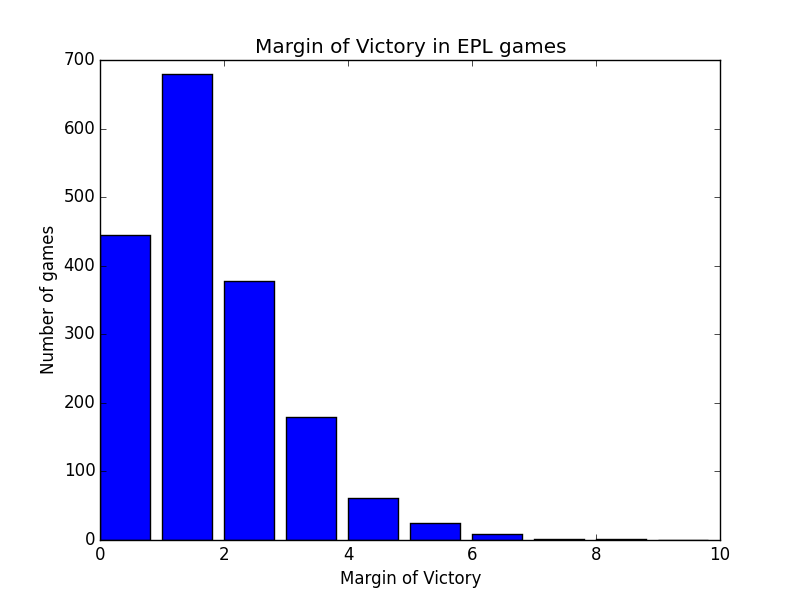
\includegraphics[width=0.7\linewidth]{MarginOfVictory}
\caption{}
\label{fig:MarginOfVictory}
\end{figure}


Finding free to use data sources was difficult. Many sports betting sites do not give out their stats for teams and many sports website either do not have APIs or do not have free to use APIs. We were finally able to find a free to use website that contained all the information we were looking for. This website was described in the previous section.

Another difficult factor of soccer games is the nature of how close they are. Fig. 1. shows the margin of victory of EPL games and this is over several seasons. The fact that games are so close and on average separated by 1 goal, makes game prediction very difficult.


The next thing we had to do was gather the data so that we can use it. To do this, we created a python program that gathers the data from the csv files. This program allowed us to use the data to make predictions. The stats from a given season are loaded into a $\mathtt{Season}$ object, which can be queried for stats for any given team or the league at any date in the season. For example, you can request the number of points that a team has on a given date, or the standings of the league, and the object will ensure that it does not use any future data. The $\mathtt{Season}$ object can be expanded to include more features, and serves as the interface between the raw data and our developed code. Additionally, a $\mathtt{Predictor}$ object has been created which uses features from the $\mathtt{Season}$ object to predict the outcome of matches.

The first thing that we wanted to do after gathering the data was to get a baseline for predictions by using some naive predictors. The first naive predictor will always predict that the home team wins and another will always predict that the away team wins. Another predictor will always pick the team that is higher in the standings to win and another will predict the winner based on the win/loss record of the team's previous games. If a team has won a majority of its last games, we will predict it to win. If a team has lost a majority of its last games we will predict it to lose. If we predict both teams to win or both teams to lose, then we will predict a draw. The last naive predictor that we used always picked the winner based on who the betting odds predicted to win. Since the betting odds are made by professionals, we wanted to compare all our predictors against it to see how well we could do compared to the professionals.

For a machine learning algorithm we used a decision tree. We wanted to compare how well the machine learning algorithm did compared to the naive algorithms. We used Leave One Out Cross Validation where one season was left out as testing data.

Relegations effect was also explored. This began by calculating a custom statistic to represent a team's closeness to relegation. This statistic was calculated for each team in a match with reference to the match itself. This approach was chosen to represent that a low amount of points at the beginning of the season should not bring a team as close to relegation as a low amount of points at the end of the season.

For each match in the dataset, the away team and home team had their pre-match closeness to relegation calculated as: R = (Pc - Pt) / (Pm), where Pc is the points the team currently has, Pt is the theoretical maximum points available to the team in the season, and Pm is the maximum amount of points a team can achieve in a season. 

We chose to use the theoretical maximum remaining points rather than the probably amount of remaining points in this calculation to represent a team's optimistic view of the future. In essence, we believe that humans are simultanously hopeful and naturally bad statiticians, and therefore we think that teams would take the view that the amount of points remaining to them is the theoretical maximum (the amount they would achieve if they won all upcoming games). 

This gave as value for R, our closeness to relegation statistic, which ranged between 0 and 1. To test the effect the threat of relegation has on how well teams played we created four data sets. The first two sets were created from first removing all but the HomeTeam, AwayTeam, and FTR columns from our data, and then duplicating the set and appending the R calculation for each team. The second two sets were created in a similar matter from a different seasons data.

With these data sets we trained an SVM classifier. First we trained the classifier on the 14-15 season data and used it to predict the 15-16 season. Second, we trained on the appended 14-15 season data and used it to predict the appended 15-16 season's outcomes.

Since the EPL points system is an important feature in correctly predicting the outcome of a match, we decided that we would look into improving this feature as well. We wanted to look into awarding points to a team based on the margin of victory. If a team wins by a large margin, we thought that that team should be awarded more points than a team that wins by one goal. If a team wins by a large margin than that shows that that team was clearly better. If a team wins by one goal than that shows that that team may only be slightly better than the other team. Our point system would also give points to the losing team. If a team loses by one goal then they should get more points than a team that loses by many goals.

\section{Results}

 Naive predictors have been programmed to determine a baseline. One predictor always chooses the home team, one always chooses the away team. One always predicts the team higher in the standings, and one predicts based only on whether teams had won or lost their last game. We also created a predictor that always chooses the winner based on who has the better betting odds. The machine learning algorithm that we use was a decision tree and was found to be more accurate that the naive predictors. The results are shown below over five seasons of EPL soccer.

\begin{center}
  \begin{tabular}{@{} cc @{}}
    \hline
    Predictor & Accuracy \\ 
    \hline
High Points & 0.456599190283 \\ 
    Last Game & 0.381983805668\\ 
    Home Team & 0.43979757085 \\ 
    Away Team & 0.308259109312\\ 
    Betting Odds & 0.525829959514\\
    Decision Tree & 0.534736842105\\
    \hline
  \end{tabular}
\end{center}

It is note worthy how well a home-team predictor performs, rivaling a high-points predictor, and confirming that home field advantage in EPL soccer.

A simple decision tree machine learning approach was used, using LOOCV where one season was left out as testing data. Limiting the depth of the tree improved results and avoided over fitting, but the accuracy was not much better than the high-points model. This indicates that more advanced features need to be used, most obviously score.

Fig. 2. shows how each of the predictors compare against each other. 

For the effect of relegation. The accuracy of predictions without relegation was 36.15\% while the accuracy with the relegation data was 36.53\%. This represented only a slight increase (0.4\%) in predictive power when a team's closeness to relegation was taken into account.

\begin{figure}[t]
\centering
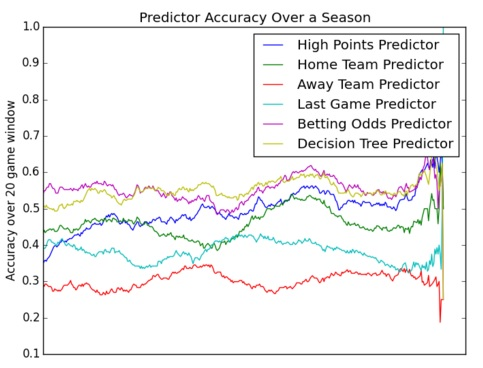
\includegraphics[width=0.7\linewidth]{graph}
\caption{}
\label{fig:graph}
\end{figure}

\section{Custom Points Scoring System}
As EPL points was shown to be the most important feature in correctly predicting the outcome of a match, we decided to improve upon this feature. Awarding three points for a win and one point for a draw is would seem like a fairly arbitrary decision, and could be improved upon, as it does not incorporate margin of victory, and also restricts itself to integer numbers. We set to learn a better point system that would award teams based on the margin of victory, giving a certain number of points for a draw, a win by one point, a loss by one point, a win by two points etc. Mathematically, we represent a team's record by a vector $R$, and the total number of points is calculated by taking the dot-product of $R$ with the scoring vector $S$. For example, in the existing EPL points system $S=[0, 1, 3]$, representing 0 points for a loss, 1 point for a draw and 3 points for a win. A team with 2 losses, 1 draw, and 3 wins $R = [2,1,3]$ would then have $S \cdot R = 10$ points. First we extended the granularity of these vectors by increasing their size to represent wins and losses by $>2$ points, 2 points, and 1 point, as well as a draw, giving $R$ and $S$ both a length of 7. 

The goal of this new scoring system is to better order the teams in a ranking. A perfect ranking does not exist, which can be easily shown by there not being a undefeated team in any of the season -- in other words there is no team that is better against all teams. Instead this is to try to determine a ranking (or ordering) of the teams that is better than the existing standings system. The parameters of $S$ were trained using the following model:

Given a home team with the record $R_{home}$ and an away team with the record $R_{away}$, predict a home team victory if the home team's season standing points are higher than the away teams ($S \cdot R_{home} > S \cdot R_{away}$), otherwise pick the away team to win.

Rearranging the condition for predicting the home team:\\$S \cdot R_{home} - S \cdot R_{away} > 0$\\
$S \cdot (R_{home} - R_{away} ) > 0 $\\
Setting the game vector, $G$ to $G = R_{home} - R_{away}$ it becomes clear that this model of classification is identical to a linear perceptron, and so to train a linear perceptron is to learn the parameters in $S$. 

The perceptron was trained using only instances of games which had a winner, in order to make this a binary classification model, and using season-end records for each team instead of game-day records to prevent the cold start problem at the start of the season. Prediction accuracy was found to be around 65\% after running for 2000 iterations, varying slightly depending on the initial conditions. Surprisingly, the perceptron often learns a positive association with 3 goal loss, more so often than a one point loss or a draw. We believe this merely suggests that good teams lose by larger margin of victory more often than bad teams do. When the data is normalized (the game vector $G$ made to have a length of 1), prediction accuracy increases to 69\%, and a no positive association with a three goal loss was found, however a negative association was often found for two goal wins. This was considered to be a sign of overfitting, that not enough games in the dataset were won by large point margins, and so the record vectors were reduced to a size of 5, including $>1$ and $1$ point win/losses, and draws. This resulted in increasing values for each margin of victory, but resulted in a slight drop in prediction accuracy to 67\%. As every game vector is calculated $R_{home} - R_{away}$, the bias term learned by the perceptron represents the home field advantage. 

An example of the learned $S$ vector = $[-0.9860, -0.6646, -0.5614,  0.3972,  0.4145]$, and the bias term $=0.16079869$.

At the end of the season, however, it is found that this new learned points system did not have significant impact on the standings. The majority of teams in the 2014/15 season (11/19 teams) placed exactly the same under the new points system, with the other 8 teams differing by at most one position, as can be seen in Table \ref{tab:standings}. 


\begin{table} [h]
	\caption{End of season standings under old and new scoring systems for the 2014-15 season}
	\label{tab:standings}
	\begin{center}
		\begin{tabular}{@{} ccc @{}}
			\hline
			Team & Old points& New points \\ 
			\hline
			Chelsea  &  1  &  1 \\
			Man City  &  2  &  2 \\
			Arsenal  &  3  &  3 \\
			Stoke  &  4  &  4 \\
			Man United  &  5  &  5 \\
			Tottenham  &  6  &  6 \\
			Everton  &  7  &  7 \\
			Hull  &  8  &  8 \\
			Liverpool  &  9  &  10 \\
			Southampton  &  10  &  9 \\
			West Brom  &  11  &  12 \\
			QPR  &  12  &  11 \\
			Leicester  &  13  &  13 \\
			Sunderland  &  14  &  15 \\
			West Ham  &  15  &  14 \\
			Swansea  &  16  &  17 \\
			Aston Villa  &  17  &  16 \\
			Crystal Palace  &  18  &  18 \\
			Newcastle  &  19  &  19 \\
			Burnley  &  20  &  20 \\
			\hline
		\end{tabular}
	\end{center}
\end{table}

%still more to do here
\section{Conclusion and Future Work}
Predicting the outcome of matches in the EPL has proven to be difficult due to closeness of games, lack of scoring, and the way that the EPL points system is set up. 

Using our naive algorithms, we were able to get a prediction of accuracy of around 50\% with the decision tree algorithm having the best result of about 53\% prediction accuracy. 

While investigation the effect of relegation on a team's performance it was found that closeness to relegation has negligible increase on the predictive power of SVM classifiers over the EPL data. We only saw a 0.4\% increase in the prediction accuracy when taking into account relegation.

By adjusting the scoring system of the EPL, we were able to get more accurate results. By using a linear perceptron algorithm, we were able to get a prediction accuracy as accurate as 69\%. However, at the end of the season it was found that the new point system had a minimal change on the standings compared to the current EPL point system.

Future work will look at the following tasks that we would like to complete.\begin{center}
 \begin{tabular}{@{} cc @{}} 
   \hline
       -Find most accurate machine-learning model\\ 
       -Use our relegation feature in more models\\  
       %Learn a more accurate points system\\ 
   \hline
 \end{tabular}
\end{center}
\hfill

%We are measuring a team’s closeness to relegation as a normalized number (0.0, 1.0)
%\begin{center}
 %\begin{tabular}{@{} cc @{}} 
%   \hline
%0 means no chance of relegation\\
%1 means high chance of relegation\\
%\hline
% \end{tabular}
%\end{center}
%Measure in this case will be derived from this formula
%\begin{center}
%Measure:  team pts + theoretical max remaining pts / max pts.
%\end{center}

%Where $\mathtt{points}$ is the current number of points that the team has so far in the season and $\mathtt{team\_max\_points}$ is the maximum number of points a team can get based on the number of games they have left in the season. The higher the relegation score, the closer the team is to relegation. This relegation score formula may still need to be improved.
There are more algorithms that we want to create to try and get more accurate prediction results. We want to create an algorithm that determines the outcome of the game by looking at the team's last X number of games. We will want to find an X that will provide the most accurate results. For example, if team A has won 3 of its last 5 games and team B has won 1 of its last 5 games then we will predict that team A will win the game. If it is predicted that both teams will win or both teams will lose, then we will predict a draw for that game. We will run this algorithm for different number of X games to find the X that gives the most accurate results. We will compare these results with the results of the naive algorithms to see if there are any improvements.
We also want to try more of our algorithms with our relegation score taken into account. We will run our other algorithms with the relegation score and without the relegation score to see if there are any differences in the outcomes. This will give more evidence to see if a team being in relegation will affect the outcome of the match or not. 

\section{Task Breakdown}
Kolby and Alastair worked together to do the write ups for the project reports and help out with some of the code. This sub-team also collected all the data for this project using the website and methods explained in Data Description. This sub-team focused on making sure the group was meeting the proper deadlines and helping out with the coding and machine learning aspects when the other sub-team needed help. Kolby and Alastair also coded the betting odds into the graph so we could have a baseline for our algorithms to be compared to.

Graeme and Cole worked on creating python scripts and training the machine learning algorithms on the data. This sub-team trained our decision tree and also the other predictors and created a graph for the results of these predictors based on our data. These two sub-teams worked very well together as we could easily delegate tasks to each other to meet our deadlines. Since most of our scripts were not too challenging, either Graeme or Cole would be assigned to complete these tasks and then we would all check to make sure it generated the results we needed.

In terms of writing the report Cole completed the Related work section and got the team starting in doing research on past projects relating to ours. The main reason as to why we had such a strong start on how to accomplish our task at hand was due to Cole's extensive research into the related work. Graeme helped complete the approach section as he mainly focused on the relegation statistic and factoring relegation into our algorithms and learning models. Being the expert on relegation all parts of the report relating to that were completed by Graeme. 

Every member of the team would be involved in the decision for deciding our next step and the work was evenly distributed between each member, if Cole and Graeme was working on more scripts, Alastair and Kolby would be working on adding more functionality to the scripts or documenting the changes in our reports to keep track of what is happening. This project was a success due to the high work ethic of every team member and the separation of tasks into sub tasks that each sub-team could tackle with ease. 

\nocite{*}

% can use a bibliography generated by BibTeX as a .bbl file
% BibTeX documentation can be easily obtained at:
% http://mirror.ctan.org/biblio/bibtex/contrib/doc/
% The IEEEtran BibTeX style support page is at:
% http://www.michaelshell.org/tex/ieeetran/bibtex/
\bibliographystyle{IEEEtran}
% argument is your BibTeX string definitions and bibliography database(s)
\bibliography{b}

% that's all folks
\end{document}


